%! TEX root = ../main.tex
% =============================================================
% IMMUTABLE — generated automatically, do not edit this block
%   script          : analysis_scratch/probe_height_figure.py
%   plot_type       : probe_height
%   chapter         : 04
%   conditions      : cond1 h272/high, cond2 h136/high, cond3 h100/high (WRONG), cond4 h100/low
%   probes          : 9373/170, 12400/250, 9373/340, 8804/250
%   sw_n_total      : 43
%   wind_n_total    : 16
% =============================================================
\begin{figure}[htbp]
  \centering
  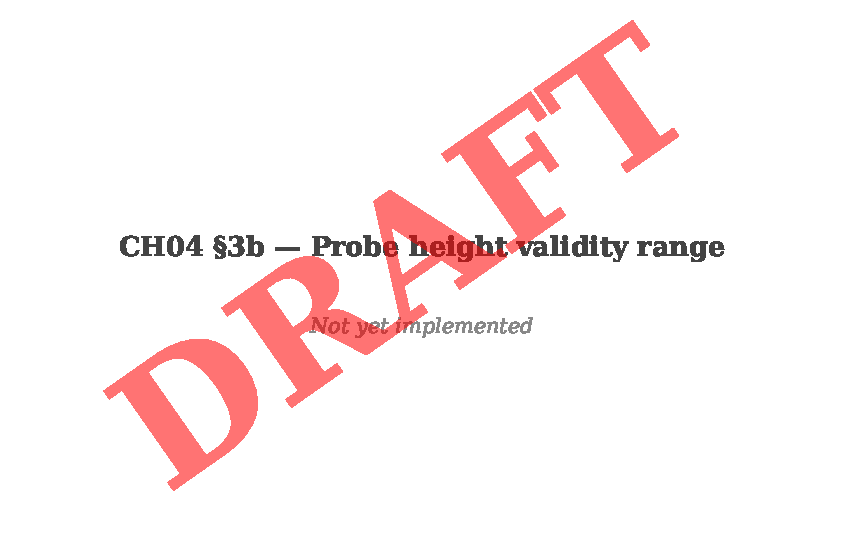
\includegraphics[width=0.98\linewidth]{FIGURES/ch04_probe_height.pdf}
  \caption[Probe height and range-mode validity]{%
    Stillwater noise floor (a) and wind-background amplitude (b) per probe, for the four hardware configurations encountered during the experiment: cond1 ($h\!=\!272$\,mm, high-range, standard), cond2 ($h\!=\!136$\,mm, high-range, $n\!=\!1$ stillwater), cond3 ($h\!=\!100$\,mm, high-range — wrong mode: $h$ is below the $130$\,mm window minimum), and cond4 ($h\!=\!100$\,mm, low-range — correct, used for all CH05 results). Bars: mean across nowave runs in each group (errorbars: $\pm 1\,\sigma$ where $n\!>\!1$). At the IN probe, lowering the probe drops the stillwater noise from $\sim\!289$\,$\mu$m (cond1) to $\sim\!102$\,$\mu$m (cond4) — the longer acoustic path of cond1 contributes more drift and attenuation. The OUT probe is sheltered by the panel geometry, with wind-background $\sim\!0.91$\,mm vs $\sim\!10.6$\,mm at the IN probe — a $\sim\!10\times$ reduction. Dashed segments in (a): detection threshold $2\times$ max-condition noise floor per probe. Note: cond3 is the source of the P2-probe-malfunction runs flagged by the pipeline quality system.
  }
  \label{fig:ch04_probe_height}
\end{figure}
